\section{Manejo de Guardas: \\ Guard Providers}
\label{sec:guard_providers}
Las guardas permiten relacionar la RdP con el estado del medio, y representar
condiciones de ejecución síncronas propias del mismo sistema (ver
secciones~\ref{sec:arquitectura_alto_nivel} y ~\ref{guardas}).

El monitor de Petri ofrece una interfaz para establecer el valor de una guarda.
De esta manera se permite al usuario indicar directamente dicho valor. Sin
embargo, el uso de esta alternativa trae aparejada una pérdida de la inversión
de control debido a que se modifica el estado de la red de manera directa y en
cualquier instante, permitiendo al usuario tomar decisiones sobre el control del
flujo de ejecución.

Para lidiar con este problema se propone el concepto de Guard Provider. Un Guard
Provider es un método asociado a una guarda que retorna una variable de tipo
boolean. Este método es llamado automáticamente por el framework luego de
ejecutar un controlador de acción que requiera modificar dicha guarda. Para
lograr la llamada automática a un Guard Provider se utiliza reflection (ver
sección~\ref{reflection}). El método Guard Provider retorna el valor que debe
tomar la guarda asociada.

El concepto de Guard Provider permite limitar el acceso a las
guardas. En consecuencia, la modificación de una guarda se realiza sólo tras
la ejecución de las acciones que deben modificar en la RdP el estado
representado por dicha guarda. El usuario tiene la capacidad de definir la
lógica que dará el valor a la guarda, pero el monitor conserva la decisión de
ejecución del Guard Provider, ya que la misma esta asociada a la ejecución de
los controladores de acciones (ver sección~\ref{sec:controladores_de_acciones})

\begin{figure}[H]
	\centering
	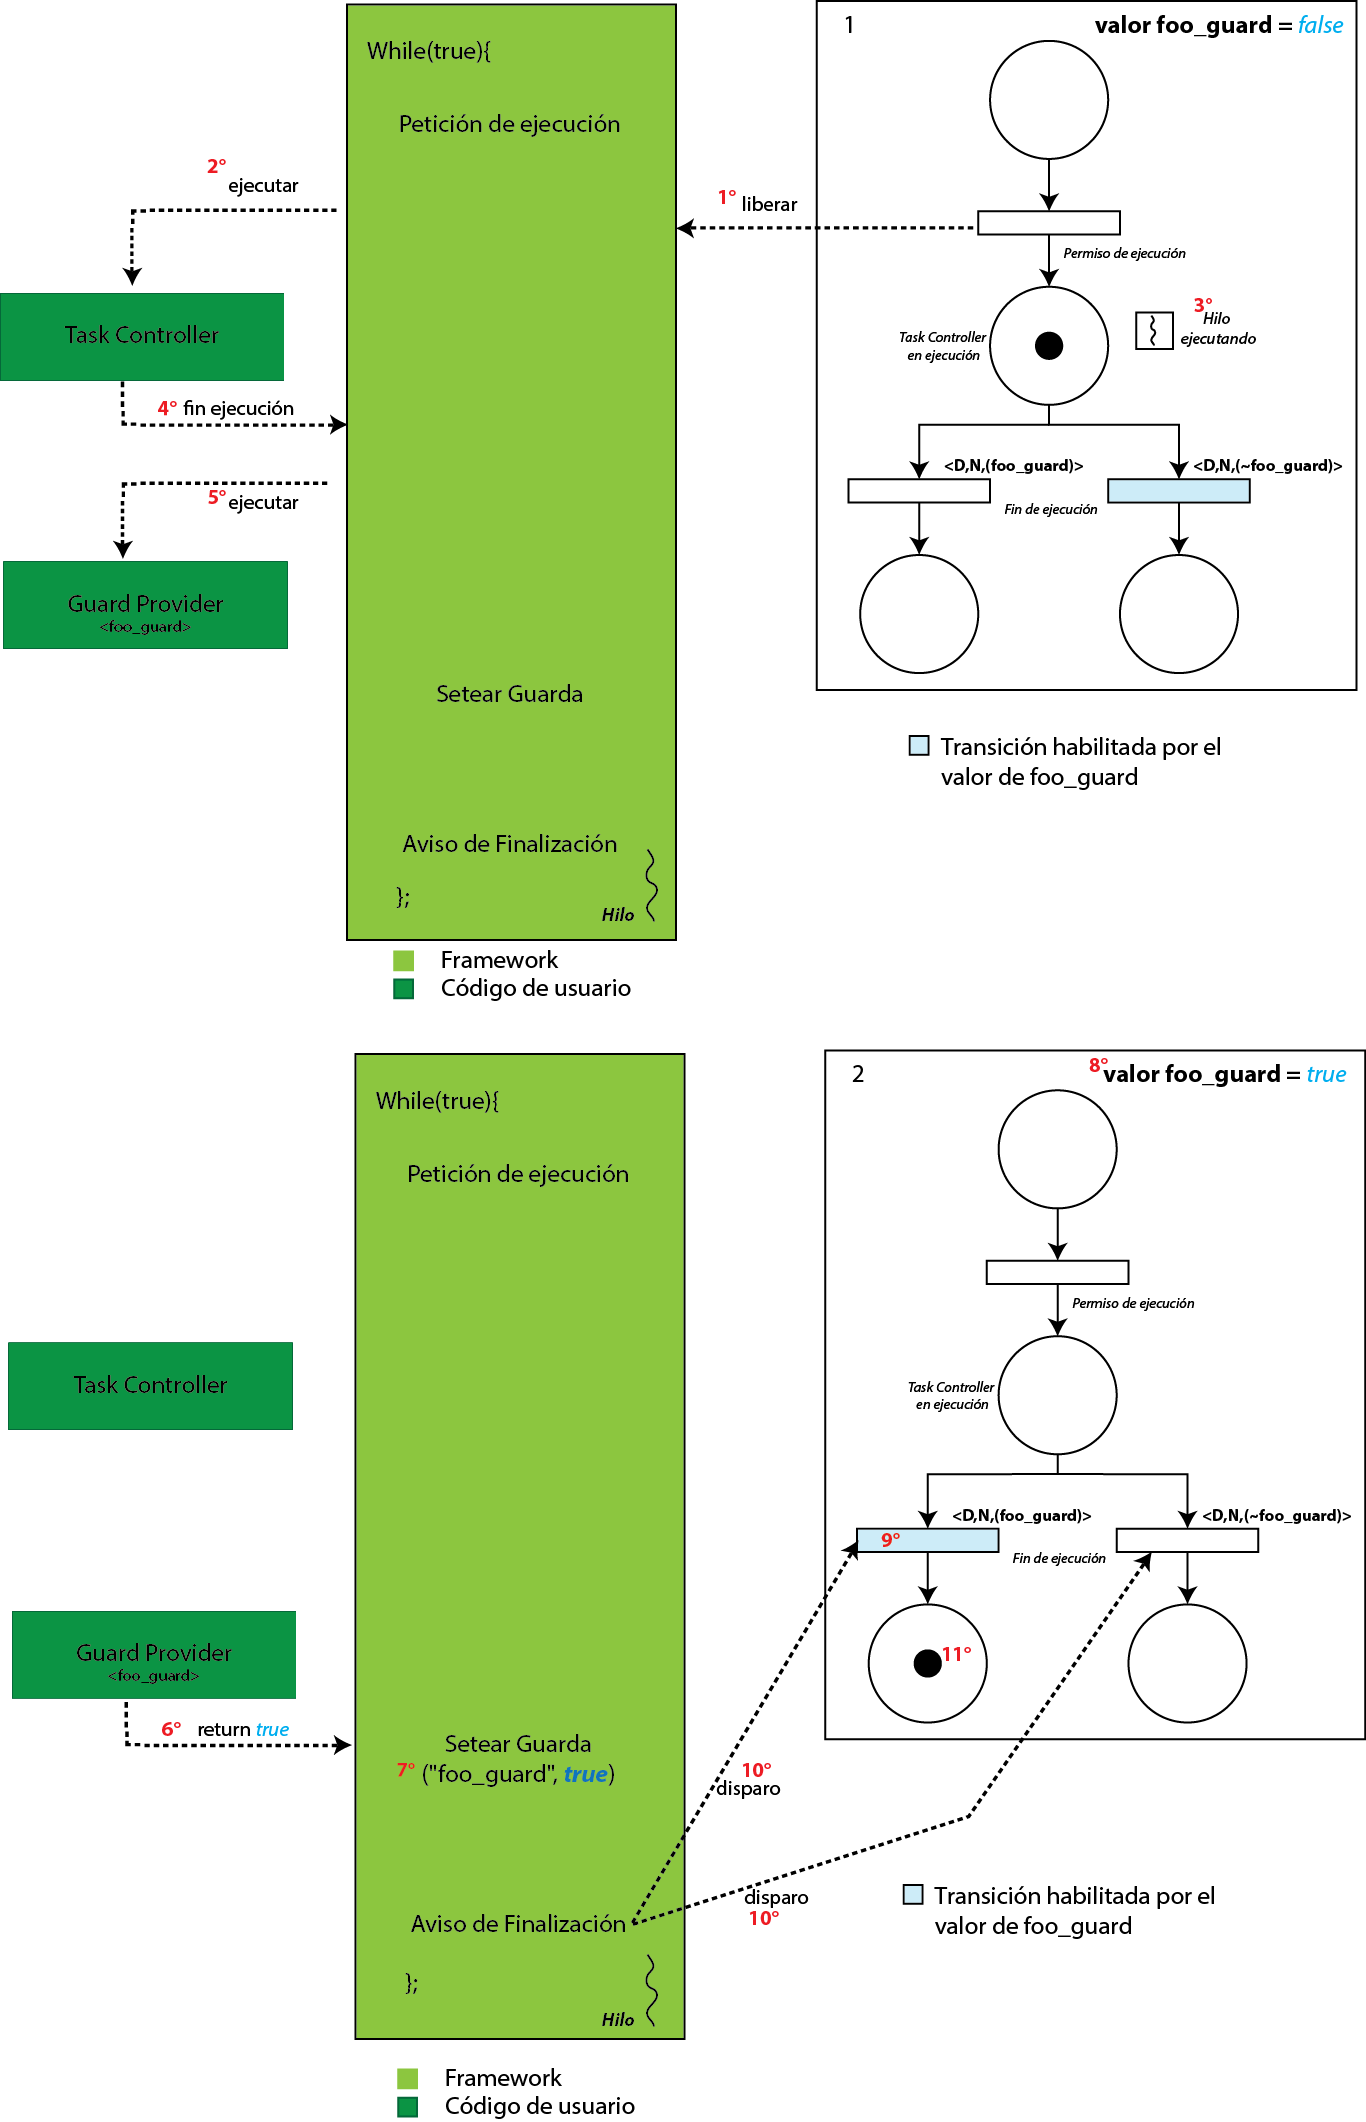
\includegraphics[width=0.9\textwidth]{ejecucion_guard_provider}
	\caption{Pasos de la Ejecución de un Guard Provider asociado a un Task
	Controller }
	\label{fig:ejecucion_guard_provider}
\end{figure}